\chapter{Tổng kết và hướng phát triển}

\section{Tổng kết}
Bài tập lớn ``CyberCAN Defense - Phát hiện và phòng thủ xâm nhập mạng nội bộ ô tô'' tập trung nghiên cứu giao thức CAN, phân tích các điểm yếu bảo mật đặc trưng của bus này và xây dựng một mô hình giám sát, phát hiện, phòng thủ trên nền tảng ESP32 \cite{bosch-can20,koscher2010,miller2015}.

Trong quá trình thực hiện, nhóm đã đạt được các kết quả nổi bật sau:
\begin{itemize}[leftmargin=*]
    \item \textbf{Nghiên cứu lý thuyết nền tảng:} Nhóm đã hệ thống lại các kiến thức quan trọng về CAN như cấu trúc khung dữ liệu, cơ chế phân xử ưu tiên, truyền thông broadcast, phát hiện lỗi và yêu cầu lớp vật lý của bus \cite{bosch-can20}.
    \item \textbf{Xây dựng mô hình hệ thống CAN thực tế:} Sử dụng các bo mạch vi điều khiển ESP32 và các module CAN của nhóm (dùng transceiver TJA1050 hoặc phần cứng tương đương), nhóm đã thiết lập mô hình bus CAN hai chiều giữa nhiều nút và máy tính giám sát \cite{espressif-twai,nxp-tja1050,bosch-can20}. Firmware được triển khai theo hướng gọn nhẹ, dễ kiểm thử và bám sát phần cứng thực tế của mô hình.
    \item \textbf{Thiết kế hệ thống truyền nhận cơ bản và có bảo vệ:}
    \begin{itemize}
        \item Luồng truyền nhận CAN cơ bản được xây dựng để mô phỏng hoạt động bình thường giữa các nút trong mạng \cite{koscher2010,miller2015}.
        \item Luồng có bảo vệ tích hợp bộ đếm thông điệp, phát hiện lặp khung, phát hiện ngập lưu lượng và cơ chế chặn theo CAN ID khi có cảnh báo \cite{koscher2010,miller2015}.
    \end{itemize}
    \item \textbf{Mô phỏng tấn công và phòng thủ:}
    \begin{itemize}
        \item Hệ thống hỗ trợ mô phỏng các kịch bản replay, spoofing theo chu kỳ và spam/DoS thông qua các lệnh điều khiển trên terminal \cite{koscher2010,miller2015}.
        \item Cơ chế phòng thủ cho phép phát hiện bản tin bất thường và cô lập tạm thời các CAN ID bị nghi ngờ ở mức ứng dụng \cite{koscher2010,miller2015}.
    \end{itemize}
    \item \textbf{Xây dựng giao diện trực quan bằng website:} Ứng dụng web dùng FastAPI, WebSocket và kết nối serial để theo dõi bản tin CAN, hiển thị cảnh báo, điều khiển tấn công và kích hoạt phòng thủ từ giao diện tập trung \cite{fastapi-docs,pyserial-docs}.
    \item \textbf{Minh họa kết quả qua thực nghiệm:} Mô hình phần cứng và phần mềm của đề tài cho thấy khả năng trình diễn rõ ràng luồng truyền CAN cơ bản, kịch bản tấn công và phản ứng của cơ chế bảo vệ trên cùng một hệ thống.
\end{itemize}

Kết quả của dự án cho thấy cách tiếp cận phát hiện bất thường kết hợp chặn theo ID có thể nâng cao khả năng quan sát và giảm tác động của các bản tin nghi ngờ trong mô hình CAN thử nghiệm \cite{koscher2010,miller2015}. Đây là nền tảng phù hợp để tiếp tục phát triển các cơ chế bảo mật mạnh hơn cho mạng truyền thông nội bộ ô tô.

\section{Ứng dụng Trí tuệ Nhân tạo (AI)}

Trong quá trình thực hiện dự án CyberCAN Defense: Phát hiện và Phòng thủ Xâm nhập Mạng Nội bộ Ô tô, nhóm đã sử dụng nhiều công cụ Trí tuệ Nhân tạo (AI) khác nhau nhằm hỗ trợ nghiên cứu, thiết kế hệ thống, phát triển phần mềm và xây dựng tài liệu kỹ thuật. Mỗi công cụ được sử dụng cho những mục đích khác nhau dựa trên thế mạnh riêng, bao gồm ChatGPT, Claude và Prism AI. Việc kết hợp các công cụ AI đã giúp nhóm rút ngắn thời gian nghiên cứu, nâng cao hiệu quả làm việc và hỗ trợ giải quyết nhiều vấn đề kỹ thuật trong quá trình thực hiện đề tài.

\subsection{Ứng dụng ChatGPT trong nghiên cứu và thiết kế hệ thống}

ChatGPT được sử dụng chủ yếu trong giai đoạn nghiên cứu lý thuyết, tìm hiểu công nghệ và hỗ trợ thiết kế hệ thống. Trong quá trình tìm hiểu kiến thức nền tảng, ChatGPT hỗ trợ giải thích các khái niệm liên quan đến giao thức CAN Bus, cấu trúc CAN Frame, cơ chế Arbitration, Error Detection, Error Handling, Bit Stuffing cũng như nguyên lý hoạt động của bộ điều khiển TWAI trên ESP32 và bộ chuyển đổi CAN TJA1050.

Bên cạnh đó, ChatGPT còn được sử dụng để tìm hiểu các nội dung chuyên sâu về an ninh mạng ô tô, bao gồm các hình thức tấn công phổ biến trên mạng CAN như Replay Attack, Spoofing Attack, Denial of Service (DoS), Fuzzing Attack, Message Injection Attack và các phương pháp phát hiện xâm nhập đang được sử dụng trong các hệ thống IDS hiện đại. Công cụ này giúp nhóm tiếp cận nhanh với các kiến thức mới, giải thích các thuật ngữ chuyên ngành và đề xuất các hướng nghiên cứu phù hợp với phạm vi của đề tài.

Trong giai đoạn thiết kế hệ thống, ChatGPT hỗ trợ xây dựng kiến trúc tổng thể của dự án, đề xuất các phương án kết nối giữa ESP32, TJA1050, CAN Bus, Node Attacker, Node Defender và giao diện Web Monitoring. Công cụ cũng hỗ trợ xây dựng sơ đồ khối hệ thống, sơ đồ luồng dữ liệu, lưu đồ thuật toán và các sơ đồ minh họa phục vụ cho quá trình thiết kế và trình bày báo cáo. Ngoài ra, ChatGPT còn hỗ trợ giải thích kiến trúc AUTOSAR, phân tích mối liên hệ giữa dự án CyberCAN Defense và các thành phần trong AUTOSAR Classic Platform, từ đó giúp nhóm xây dựng phần đánh giá và định hướng phát triển của hệ thống theo các tiêu chuẩn công nghiệp.

Trong quá trình xây dựng báo cáo, ChatGPT được sử dụng để hỗ trợ tổng hợp thông tin từ nhiều nguồn tài liệu, giải thích các khái niệm kỹ thuật, đề xuất nội dung cho các chương báo cáo và hỗ trợ chuẩn hóa cách diễn đạt theo phong cách học thuật.

\subsection{Ứng dụng Claude trong phát triển và kiểm thử phần mềm}

Claude được sử dụng chủ yếu trong quá trình phát triển phần mềm và xử lý các vấn đề liên quan đến mã nguồn. Công cụ hỗ trợ giải thích cách sử dụng các thư viện lập trình trên ESP32, đề xuất cấu trúc chương trình và hỗ trợ xây dựng các module chức năng như truyền nhận CAN Frame, Web Server, WebSocket, giao diện giám sát thời gian thực và các cơ chế phát hiện tấn công.

Trong quá trình lập trình, Claude được sử dụng để hỗ trợ phân tích lỗi biên dịch, lỗi logic và các vấn đề phát sinh trong quá trình truyền nhận dữ liệu CAN. Công cụ hỗ trợ giải thích nguyên nhân gây lỗi, đề xuất các phương pháp khắc phục và đưa ra các gợi ý tối ưu hóa mã nguồn nhằm nâng cao tính ổn định của hệ thống. Đối với các thuật toán phát hiện tấn công, Claude hỗ trợ phân tích tính hợp lý của các điều kiện phát hiện, đánh giá độ hiệu quả của từng phương pháp và đề xuất các cải tiến phù hợp với khả năng xử lý của ESP32.

Trong giai đoạn kiểm thử, Claude được sử dụng để hỗ trợ xây dựng các kịch bản mô phỏng tấn công, đề xuất các trường hợp thử nghiệm và hỗ trợ phân tích dữ liệu CAN thu thập được trong quá trình thực nghiệm. Công cụ cũng hỗ trợ kiểm tra tính nhất quán của mã nguồn, rà soát các lỗi tiềm ẩn và đánh giá hiệu quả hoạt động của hệ thống IDS trước các tình huống tấn công khác nhau.

Ngoài ra, Claude còn được sử dụng để hỗ trợ xây dựng và hiệu chỉnh mã nguồn cho các thành phần Web Monitoring, xử lý dữ liệu thời gian thực và các chức năng hỗ trợ người dùng trong quá trình quan sát trạng thái mạng CAN.

\subsection{Ứng dụng Prism AI trong xây dựng tài liệu và thuyết trình}

Prism AI được sử dụng chủ yếu trong quá trình xây dựng báo cáo và chuẩn hóa tài liệu kỹ thuật. Công cụ hỗ trợ kiểm tra chính tả, ngữ pháp và tính nhất quán của nội dung, đồng thời đề xuất các cách diễn đạt phù hợp với văn phong học thuật và kỹ thuật.

Trong quá trình biên soạn báo cáo bằng LaTeX, Prism AI hỗ trợ xây dựng cấu trúc chương mục, đề xuất cách tổ chức nội dung, định dạng bảng biểu, hình ảnh và các thành phần trình bày khác nhằm nâng cao tính trực quan của tài liệu. Công cụ cũng hỗ trợ rà soát lỗi định dạng, đề xuất các cải tiến về bố cục và đảm bảo tính thống nhất giữa các chương trong báo cáo.

Bên cạnh đó, Prism AI còn được sử dụng để hỗ trợ xây dựng nội dung thuyết trình, đề xuất bố cục slide, cách trình bày các sơ đồ kỹ thuật, biểu đồ và các nội dung minh họa nhằm giúp quá trình trình bày đề tài trở nên rõ ràng và dễ tiếp cận hơn.

\subsection{Đánh giá hiệu quả sử dụng AI trong dự án}

Việc kết hợp ChatGPT, Claude và Prism AI trong các giai đoạn khác nhau của dự án đã giúp nhóm nâng cao hiệu quả nghiên cứu, đẩy nhanh tiến độ phát triển hệ thống và cải thiện chất lượng tài liệu kỹ thuật. ChatGPT hỗ trợ mạnh trong việc nghiên cứu lý thuyết, thiết kế kiến trúc và xây dựng sơ đồ; Claude hỗ trợ hiệu quả trong phát triển phần mềm, phân tích lỗi và kiểm thử hệ thống; trong khi Prism AI hỗ trợ chuẩn hóa báo cáo và nâng cao chất lượng trình bày tài liệu.

Tuy nhiên, các công cụ AI chỉ đóng vai trò hỗ trợ trong quá trình thực hiện đề tài. Mọi quyết định về lựa chọn kiến trúc hệ thống, triển khai phần cứng, phát triển phần mềm, xây dựng cơ chế phát hiện tấn công, thực hiện thí nghiệm và đánh giá kết quả cuối cùng đều do các thành viên trong nhóm trực tiếp thực hiện và chịu trách nhiệm.
\section{Liên hệ với kiến trúc phần mềm AUTOSAR}

\subsection{Tổng quan về AUTOSAR}

AUTOSAR (AUTomotive Open System ARchitecture) là tiêu chuẩn kiến trúc phần mềm được phát triển dành cho các hệ thống điện tử trên ô tô hiện đại. Mục tiêu của AUTOSAR là chuẩn hóa cách xây dựng phần mềm trên các ECU (Electronic Control Unit), cho phép các thành phần phần mềm được tái sử dụng trên nhiều nền tảng phần cứng khác nhau, đồng thời giảm chi phí phát triển và tăng khả năng tương thích giữa các nhà sản xuất.

Trong AUTOSAR Classic Platform, hệ thống được tổ chức theo kiến trúc phân lớp bao gồm Application Layer, Runtime Environment (RTE) và Basic Software (BSW). Application Layer chứa các chức năng điều khiển của xe như động cơ, phanh ABS, túi khí hoặc các chức năng an ninh mạng. Runtime Environment đóng vai trò trung gian cho phép các thành phần phần mềm giao tiếp với nhau mà không phụ thuộc trực tiếp vào phần cứng. Basic Software cung cấp các dịch vụ nền tảng như hệ điều hành, giao tiếp CAN, quản lý bộ nhớ, chẩn đoán lỗi và các trình điều khiển thiết bị.

\begin{figure}[H]
	\centering
	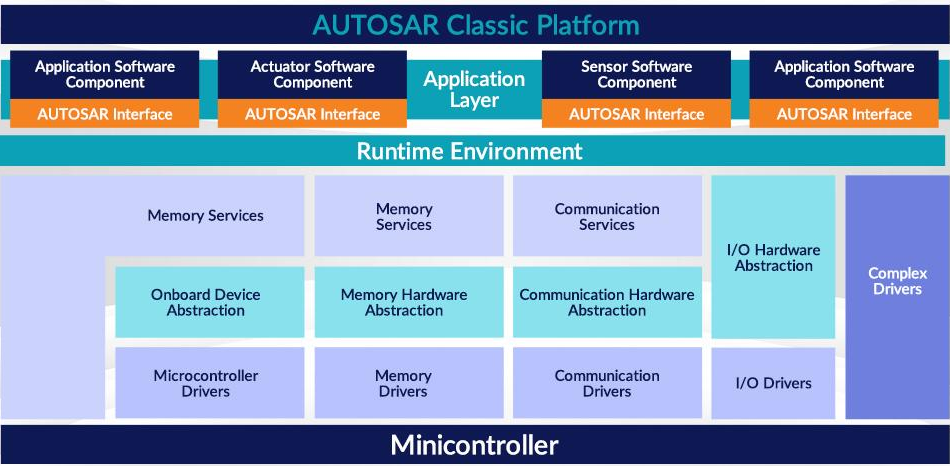
\includegraphics[width=0.75\textwidth]{images/AUTOSAR.png}
	\caption{AUTOSAR Classic Platform Architecture}
\end{figure}

Kiến trúc phân lớp này giúp tách biệt phần mềm ứng dụng khỏi phần cứng, tạo điều kiện cho việc bảo trì, nâng cấp và phát triển các chức năng mới trên xe một cách hiệu quả hơn. Hiện nay, AUTOSAR Classic được sử dụng rộng rãi trong các ECU điều khiển động cơ, hệ thống phanh, hệ thống thân xe và các hệ thống điều khiển thời gian thực trên ô tô.

\subsection{Khả năng tích hợp AUTOSAR với dự án}

Trong hệ thống, ESP32 đóng vai trò tương tự bộ vi điều khiển trung tâm của một ECU. Bộ chuyển đổi CAN TJA1050 thực hiện chức năng tương đương tầng CAN Transceiver, chịu trách nhiệm chuyển đổi tín hiệu logic từ bộ điều khiển CAN thành tín hiệu vi sai trên đường truyền CAN Bus. TWAI Driver được tích hợp trong ESP32 đảm nhiệm vai trò tương tự CAN Driver trong AUTOSAR, cho phép gửi và nhận các CAN Frame trên mạng CAN.

Bên cạnh đó, hệ thống phát hiện xâm nhập (IDS) được xây dựng trong đề tài có thể được xem như một Software Component hoạt động tại tầng Application Layer của AUTOSAR. Thành phần này tiếp nhận các CAN Frame từ mạng CAN, thực hiện phân tích dữ liệu và phát hiện các hành vi bất thường như Replay Attack, Spoofing Attack, Denial of Service (DoS) Attack và Fuzzing Attack. Khi phát hiện dấu hiệu tấn công, IDS sẽ sinh cảnh báo và gửi thông tin tới giao diện Web Monitoring để người dùng theo dõi.


\begin{table}[H]
	\centering
	\caption{Liên hệ giữa CyberCAN Defense và kiến trúc AUTOSAR}
	\label{tab:autosar_mapping}
	
	\begin{tabular}{|p{6cm}|p{6cm}|}
		\hline
		\textbf{CyberCAN Defense} &
		\textbf{AUTOSAR Classic} \\
		\hline
		
		ESP32 &
		MCU của ECU \\
		\hline
		
		TWAI Driver &
		CAN Driver \\
		\hline
		
		TJA1050 &
		CAN Transceiver \\
		\hline
			
		IDS Engine &
		Security Software Component \\
		\hline
		
		Web Monitoring Dashboard &
		Diagnostic/Monitoring Service \\
		\hline
		
	\end{tabular}
\end{table}

Từ góc nhìn của AUTOSAR, hệ thống CyberCAN Defense có thể được xem như một mô hình thu nhỏ của một ECU bảo mật trong ô tô hiện đại. Trong đó, Node Attacker mô phỏng một ECU bị xâm nhập hoặc một thiết bị độc hại được kết nối vào mạng CAN, trong khi Node Defender thực hiện vai trò giám sát và bảo vệ hệ thống. Cách tiếp cận này tương đồng với các giải pháp Intrusion Detection System đang được nghiên cứu và triển khai trong ngành công nghiệp ô tô nhằm đáp ứng các yêu cầu về an toàn và an ninh mạng theo các tiêu chuẩn hiện đại.

Trong tương lai, hệ thống có thể được mở rộng bằng cách triển khai cơ chế IDS dưới dạng một Software Component trong AUTOSAR Classic Platform hoặc tích hợp với các Security Gateway ECU. Khi đó, hệ thống không chỉ phát hiện các cuộc tấn công trên mạng CAN mà còn có khả năng phối hợp với các thành phần khác trong xe để thực hiện các biện pháp phòng thủ chủ động. Điều này giúp tăng tính thực tiễn của đề tài và tạo tiền đề cho việc nghiên cứu các giải pháp bảo mật mạng ô tô theo hướng công nghiệp.

\section{Hướng phát triển trong tương lai}
Để mở rộng tiềm năng và ứng dụng thực tiễn của dự án, nhóm đề xuất một số hướng phát triển như sau:

\begin{itemize}[leftmargin=*]
    \item \textbf{Tăng cường bảo mật với mã hóa và xác thực:} Nghiên cứu các thuật toán mật mã nhẹ hoặc mã xác thực thông điệp phù hợp với giới hạn tài nguyên của vi điều khiển và kích thước khung CAN 2.0.
    \item \textbf{Nâng cấp cơ chế phát hiện bất thường:} Mở rộng IDS theo hướng kết hợp thống kê thời gian thực với mô hình học máy để nhận biết tốt hơn các mẫu tấn công chưa xuất hiện trong tập luật hiện tại.
    \item \textbf{Tối ưu cơ chế phòng thủ:} Bổ sung chính sách chặn theo thời gian thích nghi, phân biệt mức độ nghiêm trọng của cảnh báo và tránh chặn nhầm các bản tin hợp lệ.
    \item \textbf{Phát triển dashboard thời gian thực:} Hoàn thiện giao diện giám sát với biểu đồ lưu lượng theo CAN ID, lịch sử cảnh báo và nhật ký sự kiện phục vụ đánh giá sau thực nghiệm.
    \item \textbf{Mở rộng mô hình phần cứng:} Thử nghiệm với nhiều nút hơn, nhiều loại tải hơn hoặc gateway trung gian để mô phỏng gần hơn kiến trúc mạng trong ô tô thực.
    \item \textbf{Hướng đến hệ thống đa giao thức:} Bên cạnh CAN, có thể mở rộng nghiên cứu sang LIN, CAN FD, FlexRay hoặc Automotive Ethernet để hình thành cách tiếp cận bảo mật toàn diện hơn.
\end{itemize}
